\hypertarget{poly_8cc}{
\section{poly.cc File Reference}
\label{poly_8cc}\index{poly.cc@{poly.cc}}
}
Implementation for the polynomial class. 

{\tt \#include \char`\"{}poly.h\char`\"{}}\par
{\tt \#include $<$cstring$>$}\par


Include dependency graph for poly.cc:\nopagebreak
\begin{figure}[H]
\begin{center}
\leavevmode
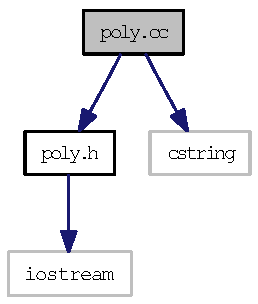
\includegraphics[width=80pt]{poly_8cc__incl}
\end{center}
\end{figure}
\subsection*{Functions}
\begin{CompactItemize}
\item 
\hyperlink{classPolynomial}{Polynomial} \hyperlink{poly_8cc_45b456660c9d558815a111d3d7c5a807}{derivative} (const \hyperlink{classPolynomial}{Polynomial} \&p)
\item 
\hyperlink{classPolynomial}{Polynomial} \hyperlink{poly_8cc_55bc2f7d47ec37dcd68435f19fa083cc}{abs} (const \hyperlink{classPolynomial}{Polynomial} \&p)
\item 
\hyperlink{classPolynomial}{Polynomial} \hyperlink{poly_8cc_aeb620028554ea52c7716904a27a7cd6}{antiderivative} (const \hyperlink{classPolynomial}{Polynomial} \&p)
\item 
std::ostream \& \hyperlink{poly_8cc_f1fdf53b29100b084772816cb9ecc8ac}{operator$<$$<$} (std::ostream \&os, const \hyperlink{classPolynomial}{Polynomial} \&p)
\item 
std::istream \& \hyperlink{poly_8cc_1446b464245742ccedeacb27fd794bab}{operator$>$$>$} (std::istream \&is, \hyperlink{classPolynomial}{Polynomial} \&p)
\end{CompactItemize}


\subsection{Detailed Description}
Implementation for the polynomial class. 

\begin{Desc}
\item[Author:]Daniel Uber \end{Desc}


Definition in file \hyperlink{poly_8cc-source}{poly.cc}.

\subsection{Function Documentation}
\hypertarget{poly_8cc_55bc2f7d47ec37dcd68435f19fa083cc}{
\index{poly.cc@{poly.cc}!abs@{abs}}
\index{abs@{abs}!poly.cc@{poly.cc}}
\subsubsection[abs]{\setlength{\rightskip}{0pt plus 5cm}abs (const {\bf Polynomial} \& {\em p})}}
\label{poly_8cc_55bc2f7d47ec37dcd68435f19fa083cc}


\begin{Desc}
\item[Returns:]absolute value of polynomial \end{Desc}


Definition at line 226 of file poly.cc.

References Polynomial::abs().

\begin{Code}\begin{verbatim}226                                    {
227   return p.abs();
228 }
\end{verbatim}
\end{Code}




Here is the call graph for this function:\nopagebreak
\begin{figure}[H]
\begin{center}
\leavevmode
\includegraphics[width=103pt]{poly_8cc_55bc2f7d47ec37dcd68435f19fa083cc_cgraph}
\end{center}
\end{figure}
\hypertarget{poly_8cc_aeb620028554ea52c7716904a27a7cd6}{
\index{poly.cc@{poly.cc}!antiderivative@{antiderivative}}
\index{antiderivative@{antiderivative}!poly.cc@{poly.cc}}
\subsubsection[antiderivative]{\setlength{\rightskip}{0pt plus 5cm}antiderivative (const {\bf Polynomial} \& {\em p})}}
\label{poly_8cc_aeb620028554ea52c7716904a27a7cd6}


\begin{Desc}
\item[Returns:]indefinite integral of p with constant 0 \end{Desc}


Definition at line 245 of file poly.cc.

References Polynomial::antiderivative().

\begin{Code}\begin{verbatim}245                                                 {
246   return p.antiderivative();
247 }
\end{verbatim}
\end{Code}




Here is the call graph for this function:\nopagebreak
\begin{figure}[H]
\begin{center}
\leavevmode
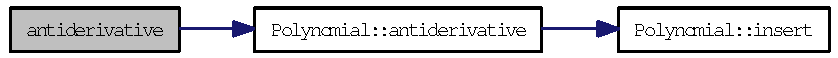
\includegraphics[width=219pt]{poly_8cc_aeb620028554ea52c7716904a27a7cd6_cgraph}
\end{center}
\end{figure}
\hypertarget{poly_8cc_45b456660c9d558815a111d3d7c5a807}{
\index{poly.cc@{poly.cc}!derivative@{derivative}}
\index{derivative@{derivative}!poly.cc@{poly.cc}}
\subsubsection[derivative]{\setlength{\rightskip}{0pt plus 5cm}derivative (const {\bf Polynomial} \& {\em p})}}
\label{poly_8cc_45b456660c9d558815a111d3d7c5a807}


return polynomial derivative 

Definition at line 209 of file poly.cc.

References Polynomial::derivative().

\begin{Code}\begin{verbatim}209                                            {
210   return p.derivative();
211 }
\end{verbatim}
\end{Code}




Here is the call graph for this function:\nopagebreak
\begin{figure}[H]
\begin{center}
\leavevmode
\includegraphics[width=201pt]{poly_8cc_45b456660c9d558815a111d3d7c5a807_cgraph}
\end{center}
\end{figure}
\hypertarget{poly_8cc_f1fdf53b29100b084772816cb9ecc8ac}{
\index{poly.cc@{poly.cc}!operator$<$$<$@{operator$<$$<$}}
\index{operator$<$$<$@{operator$<$$<$}!poly.cc@{poly.cc}}
\subsubsection[operator$<$$<$]{\setlength{\rightskip}{0pt plus 5cm}std::ostream\& operator$<$$<$ (std::ostream \& {\em os}, \/  const {\bf Polynomial} \& {\em p})}}
\label{poly_8cc_f1fdf53b29100b084772816cb9ecc8ac}


operator$<$$<$ insert polynomial into an output stream terms will be printed in order of increasing degree 

Definition at line 309 of file poly.cc.

References Polynomial::polynomial.

\begin{Code}\begin{verbatim}309                                                            {
310   Polynomial::term * t;
311   t = p.polynomial;
312   bool first = true;
313   while(t){
314     if(t->coef != 0.0){
315       if(!first)
316     os<<" + ";
317 
318       os<< t->coef;
319       if(t->deg){
320     os<<"*x";
321     if(t->deg > 1)
322       os<<"^"<<t->deg;
323       }
324       //    os<<" ";
325     first = false;
326    }
327     t = t->next;
328 
329   }
330   if (first)
331     os<<"0";
332   return os;
333 }
\end{verbatim}
\end{Code}


\hypertarget{poly_8cc_1446b464245742ccedeacb27fd794bab}{
\index{poly.cc@{poly.cc}!operator$>$$>$@{operator$>$$>$}}
\index{operator$>$$>$@{operator$>$$>$}!poly.cc@{poly.cc}}
\subsubsection[operator$>$$>$]{\setlength{\rightskip}{0pt plus 5cm}std::istream\& operator$>$$>$ (std::istream \& {\em is}, \/  {\bf Polynomial} \& {\em p})}}
\label{poly_8cc_1446b464245742ccedeacb27fd794bab}


extraction operator get a pair of numbers double, unsigned from an istream This might not be the best way to do this, and is nowhere used. 

Definition at line 340 of file poly.cc.

References Polynomial::insert().

\begin{Code}\begin{verbatim}340                                                      {
341   double coef;
342   unsigned int  degree;
343   Polynomial::term *t;
344   coef = 0.0;
345   while (coef == 0.0){
346     is>>coef;
347     is>>degree;
348     if(!is.fail()){
349       t = new Polynomial::term(coef, degree);
350       p.insert(t);
351     }
352   }
353   return is;
354 }
\end{verbatim}
\end{Code}




Here is the call graph for this function:\nopagebreak
\begin{figure}[H]
\begin{center}
\leavevmode
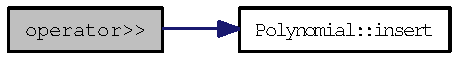
\includegraphics[width=128pt]{poly_8cc_1446b464245742ccedeacb27fd794bab_cgraph}
\end{center}
\end{figure}
